En este capítulo, se analizan los resultados obtenidos durante la implementación del proyecto de generación procedural de terrenos en Unity. Se evaluarán diferentes aspectos del proyecto y se presentarán pruebas que demuestren su funcionamiento y rendimiento.

Para la generación de estas pruebas los demás parámetros se han puesto en valores promedio para no alterar los resultados de cada una de las pruebas.

\section{Generación de Terrenos}

\subsection{Mapas de Altura Generados}

En esta sección, se presentan los resultados de la generación de mapas de altura utilizando diferentes configuraciones de parámetros. A continuación, se muestran ejemplos de cómo las variaciones en los parámetros afectan a los mapas de altura.

\subsubsection{Escala de Ruido}

La escala de ruido controla el tamaño de las características del terreno. Se han generado mapas de ruido con diferentes escalas de ruido sobre un plano para ilustrar su impacto:

\begin{figure}[ht]
    \begin{subfigure}{0.3\linewidth}
        \centering
        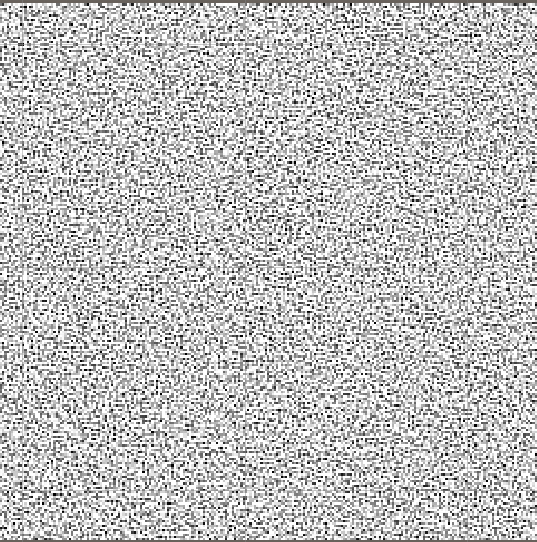
\includegraphics[width=\linewidth]{img/codes/LowNoiseScale.png}
        \caption{Escala de ruido = 1 }
    \end{subfigure}
    \hfill
    \begin{subfigure}{0.3\linewidth}
        \centering
        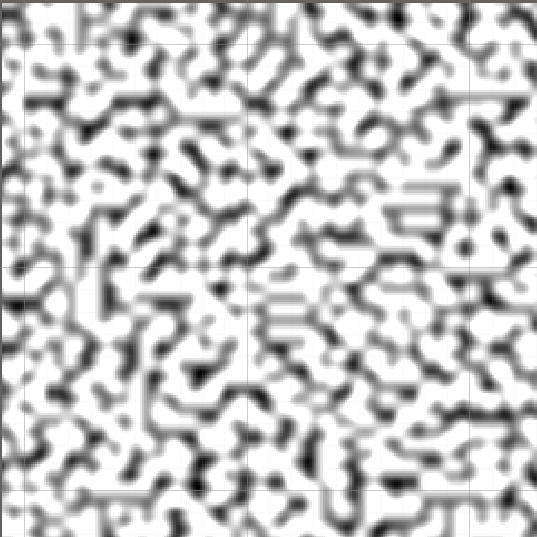
\includegraphics[width=\linewidth]{img/codes/MediumNoiseScale.png}
        \caption{Escala de ruido = 10 }
    \end{subfigure}
    \hfill
    \begin{subfigure}{0.3\linewidth}
        \centering
        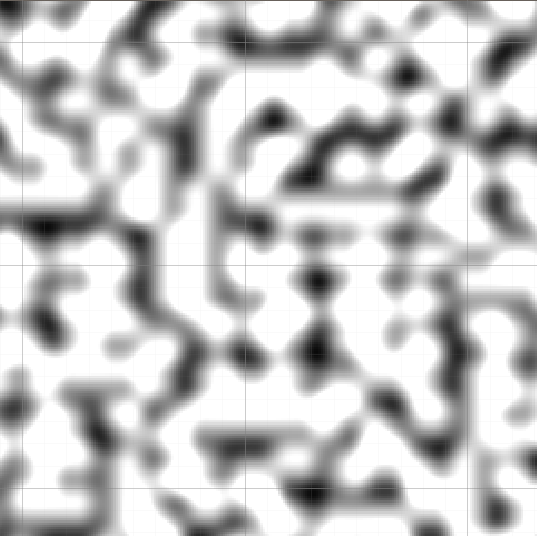
\includegraphics[width=\linewidth]{img/codes/HightNoiseScale.png}
        \caption{Escala de ruido = 20}
    \end{subfigure}
    \caption{Comparación entre valores de escala de ruido bajo, medio y alto.}
\end{figure}

Cuando la escla de ruido es pequeña se producen más detalles y más pequeños, por lo que si la escala es muy baja puede producir un exceso de ruido y dar resultados caóticos.

A medida que se aumenta la escala de ruido los detalles se hacen más amplios y se suaviza la transición entre las áreas con diferentes valores de ruido.


\subsubsection{Número de Octavas}

El número de octavas en el ruido afecta a la complejidad del terreno. Se han generado mapas de altura con diferentes números de octavas:
\begin{figure}[ht]
    \begin{subfigure}{0.3\linewidth}
        \centering
        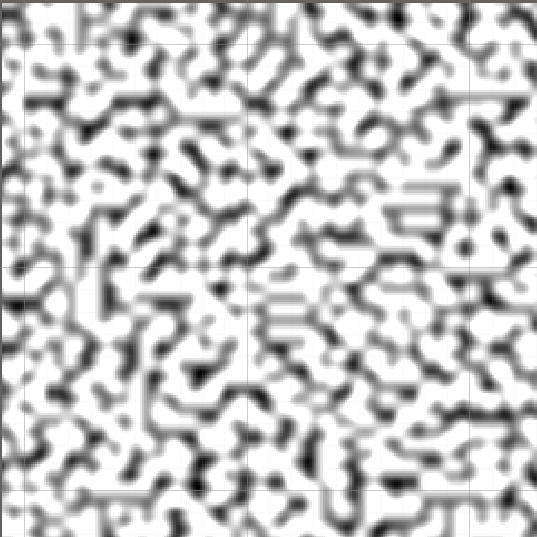
\includegraphics[width=\linewidth]{img/codes/MediumNoiseScale.png}
        \caption{Número de octavas = 1 }
    \end{subfigure}
    \hfill
    \begin{subfigure}{0.3\linewidth}
        \centering
        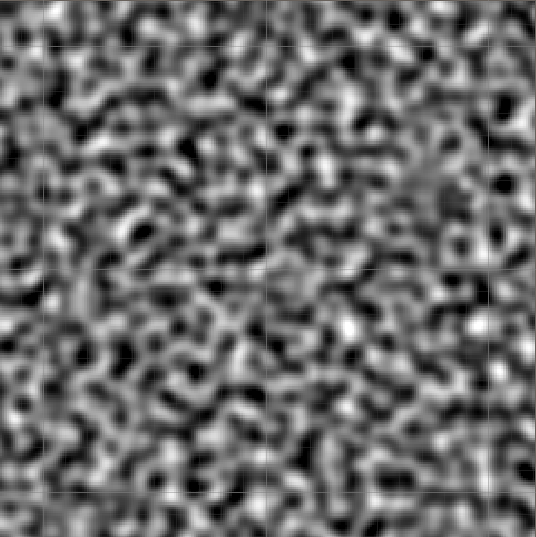
\includegraphics[width=\linewidth]{img/codes/MediumOctaves.png}
        \caption{Número de octavas = 4 }
    \end{subfigure}
    \hfill
    \begin{subfigure}{0.3\linewidth}
        \centering
        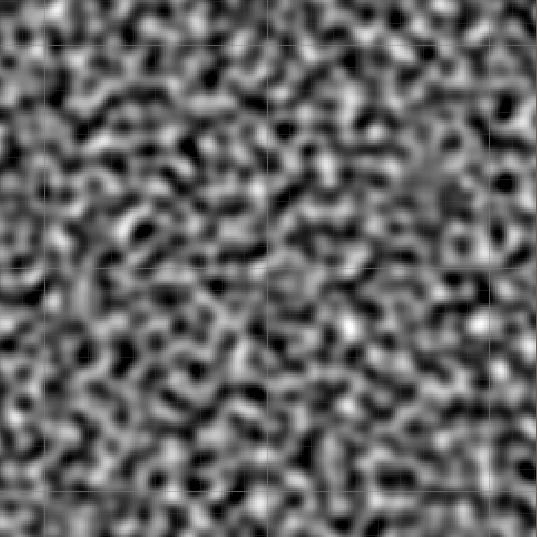
\includegraphics[width=\linewidth]{img/codes/HeightOctaves.png}
        \caption{Número de octavas = 10}
    \end{subfigure}
    \caption{Comparación entre un número de octavas bajo, medio y alto.}
\end{figure}

Como se puede comprobar, a menos Octavas, menos detalle; el patrón de ruido o textura generado tiende a ser más suave y menos detallado. Las transiciones entre valores de ruido son más graduales.
La variación en los valores de ruido es menos pronunciada, lo que resulta en menos contraste en la textura generada. La generación de ruido con menos octavas generalmente es más rápida, ya que se realizan menos cálculos.

Con más octavas, el patrón de ruido o textura es mucho más detallado y complejo. Los cambios entre valores de ruido son abruptos y pueden formar estructuras más intrincadas.
La variación en los valores de ruido es más amplia, lo que resulta en un mayor contraste en la textura generada. Generar ruido con más octavas suele ser más lento debido a la mayor cantidad de cálculos involucrados.

\subsubsection{Tipo de Ruido}

El tipo de ruido seleccionado también tiene un impacto significativo en la apariencia del terreno. Se han generado mapas de altura utilizando diferentes tipos de ruido:

\begin{itemize}
    \item \textbf{Ruido Perlin:} Se ha utilizado el ruido Perlin, que produce terrenos suaves y ondulados.
    \item \textbf{Ruido Simplex:} Se ha aplicado el ruido Simplex, que genera terrenos con detalles más naturales y menos artefactos.
    \item \textbf{Ruido de Voronoi:} El ruido Voronoi se ha empleado para crear terrenos abruptos y rugosos.
\end{itemize}

\begin{figure}[ht]
    \begin{subfigure}{0.3\linewidth}
        \centering
        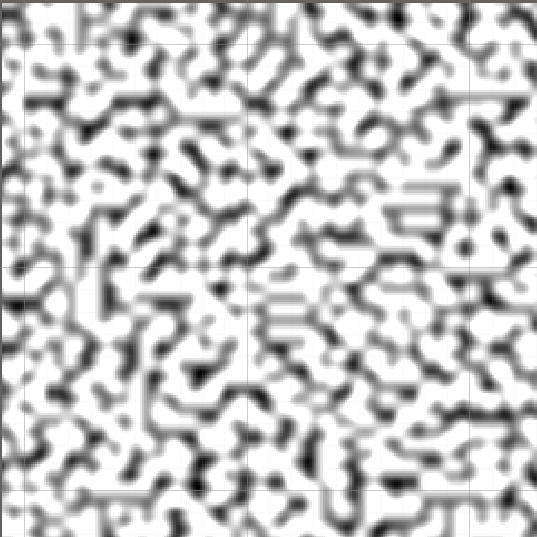
\includegraphics[width=\linewidth]{img/codes/MediumNoiseScale.png}
        \caption{Ruido Perlin}
    \end{subfigure}
    \hfill
    \begin{subfigure}{0.3\linewidth}
        \centering
        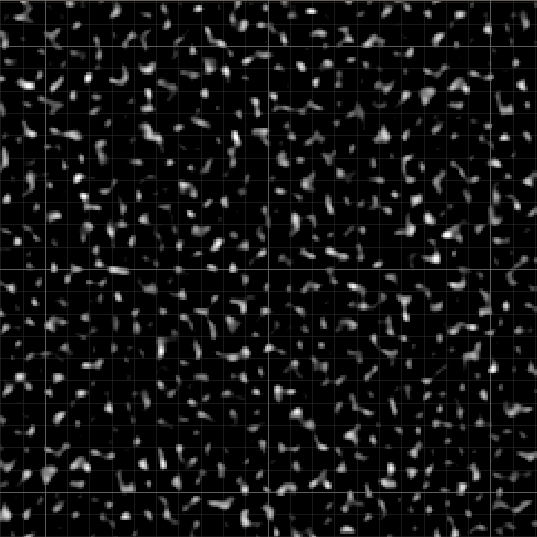
\includegraphics[width=\linewidth]{img/codes/Simplex.png}
        \caption{Ruido Simplex}
    \end{subfigure}
    \hfill
    \begin{subfigure}{0.3\linewidth}
        \centering
        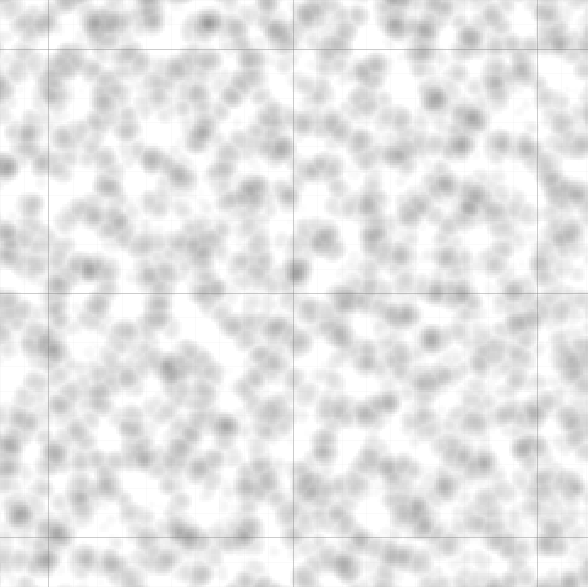
\includegraphics[width=\linewidth]{img/codes/Voronoi.png}
        \caption{Ruido Voronoi}
    \end{subfigure}
    \caption{Comparación entre generación con ruido con diferentes algoritmos.}
\end{figure}

Como se observa en las imágenes, el ruido Perlin tiene variaciones más suaves, por lo que produce terrenos más colinosos pero sin pendientes pronunciadas. En cambbio, con el Simplex, obtenemos detalles más marcados, dando lugar a áreas con detalles más marcados y áreas más llanas. Por último. Los terrenos que se obtienen con voronoi suelen ser valores altos siguiendo una estructura celular, por loq ue da lugar a terrenos escarpados e irregualres pero sin grandes pronunciaciones ya que los valores que se obitienen son más homogéneos.
\\
\\Con estos resultados variados dados por los distintos algoritmos podemos dar lugar a diferentes paisajes.

\subsubsection{Variación de Semilla de Ruido}

La semilla de ruido inicial puede afectar drásticamente la apariencia del terreno. Se han generado mapas de altura con diferentes semillas para mostrar cómo cambia el terreno:

\begin{itemize}
    \item \textbf{Semilla 123:} Mostrando el terreno generado con la semilla 123.
    \begin{figure}[ht]
        \begin{subfigure}{0.3\linewidth}
            \centering
            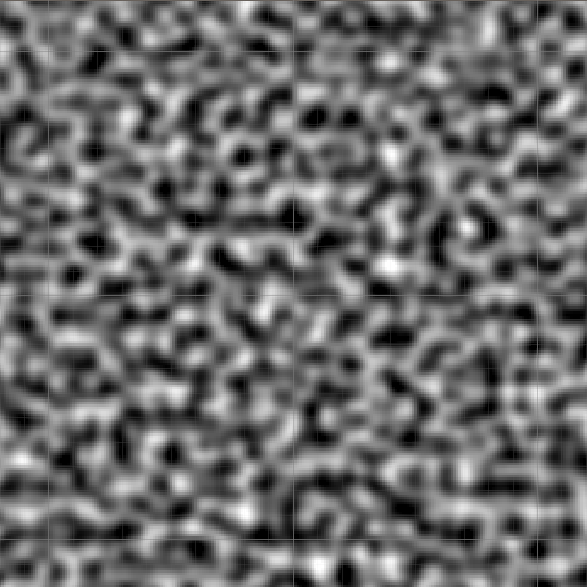
\includegraphics[width=\linewidth]{img/codes/Perlin123.png}
            \caption{Ruido Perlin}
        \end{subfigure}
        \hfill
        \begin{subfigure}{0.3\linewidth}
            \centering
            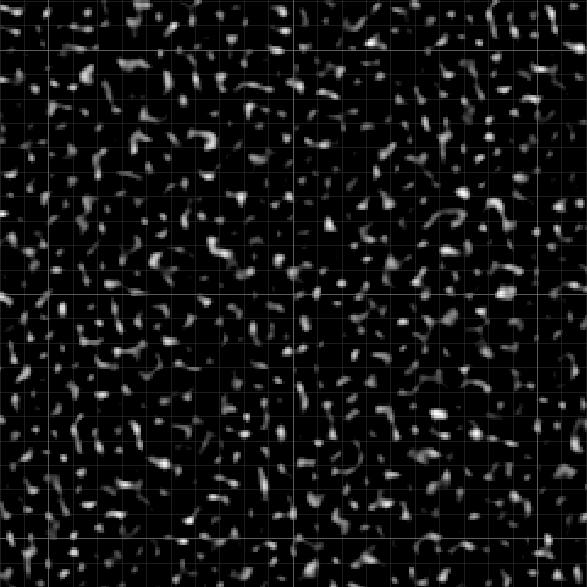
\includegraphics[width=\linewidth]{img/codes/Simplex123.png}
            \caption{Ruido Simplex}
        \end{subfigure}
        \hfill
        \begin{subfigure}{0.3\linewidth}
            \centering
            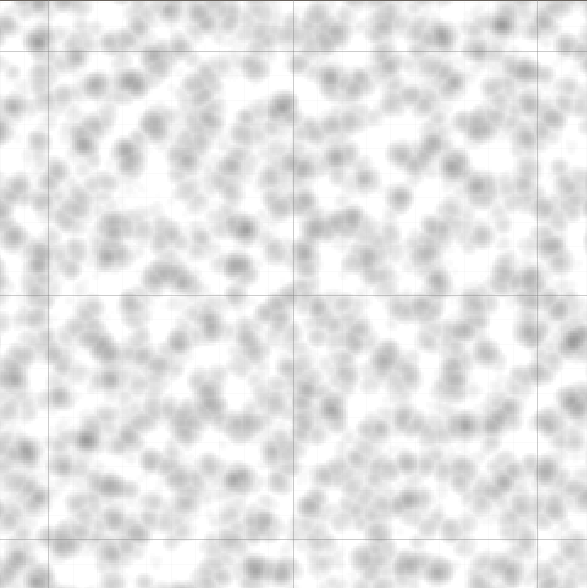
\includegraphics[width=\linewidth]{img/codes/Voronoi123.png}
            \caption{Ruido Voronoi}
        \end{subfigure}
        \caption{Ruido con los diferentes algoritmos con la semilla 123.}
    \end{figure}

    \item \textbf{Semilla 456:} Presentando el terreno generado con la semilla 456.
    \begin{figure}[ht]
        \begin{subfigure}{0.3\linewidth}
            \centering
            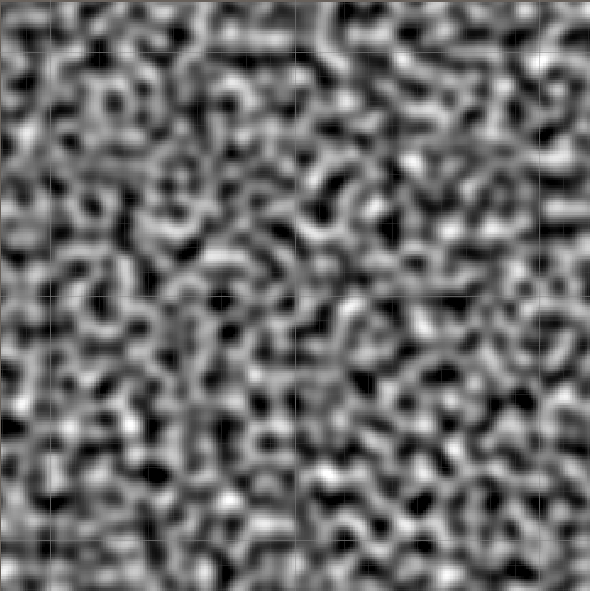
\includegraphics[width=\linewidth]{img/codes/Perlin456.png}
            \caption{Ruido Perlin}
        \end{subfigure}
        \hfill
        \begin{subfigure}{0.3\linewidth}
            \centering
            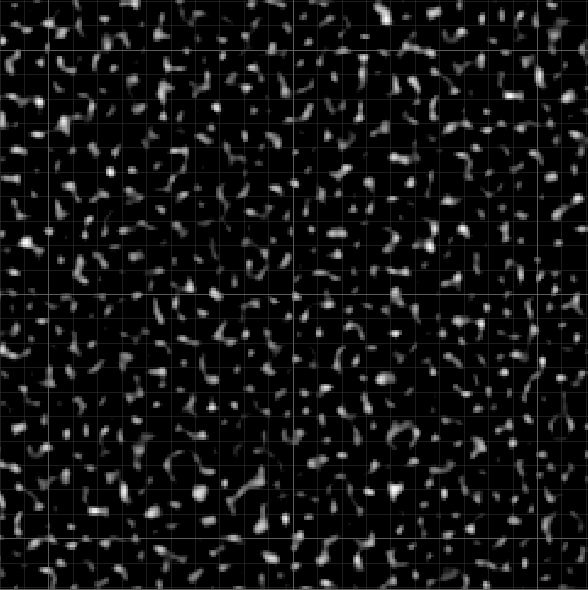
\includegraphics[width=\linewidth]{img/codes/Simplex456.png}
            \caption{Ruido Simplex}
        \end{subfigure}
        \hfill
        \begin{subfigure}{0.3\linewidth}
            \centering
            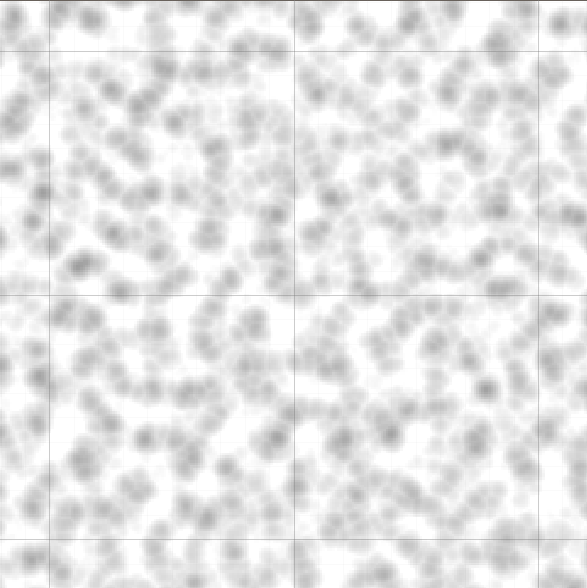
\includegraphics[width=\linewidth]{img/codes/Voronoi456.png}
            \caption{Ruido Voronoi}
        \end{subfigure}
        \caption{Ruido con los diferentes algoritmos con la semilla 456.}
    \end{figure}
\end{itemize}

\subsection{Efectos de Erosión}

\subsubsection{Ciclos: }Los ciclos representan el número de iteraciones en los que se van a recalcular las alturas de los vértices. A mayor número de ciclos, menores serán las diferencias de alturas entre los vértices.    
\begin{figure}[ht]
    \centering
    \begin{minipage}{0.4\textwidth}
        \centering
        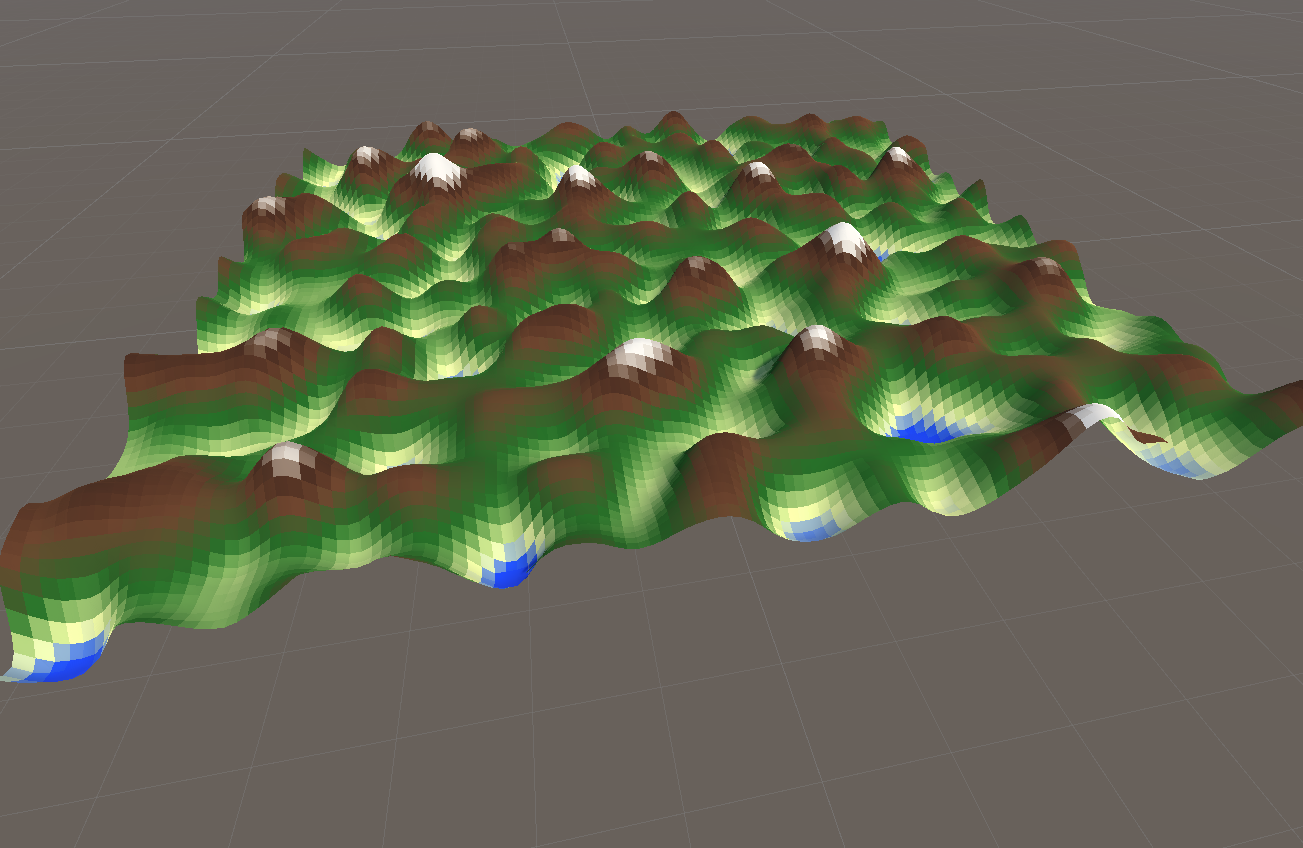
\includegraphics[width=\textwidth]{img/0ciclos.png}
        \caption{0 Ciclos de erosión, la erosión no afecta}
    \end{minipage}%
    \hfill
    \begin{minipage}{0.4\textwidth}
        \centering
        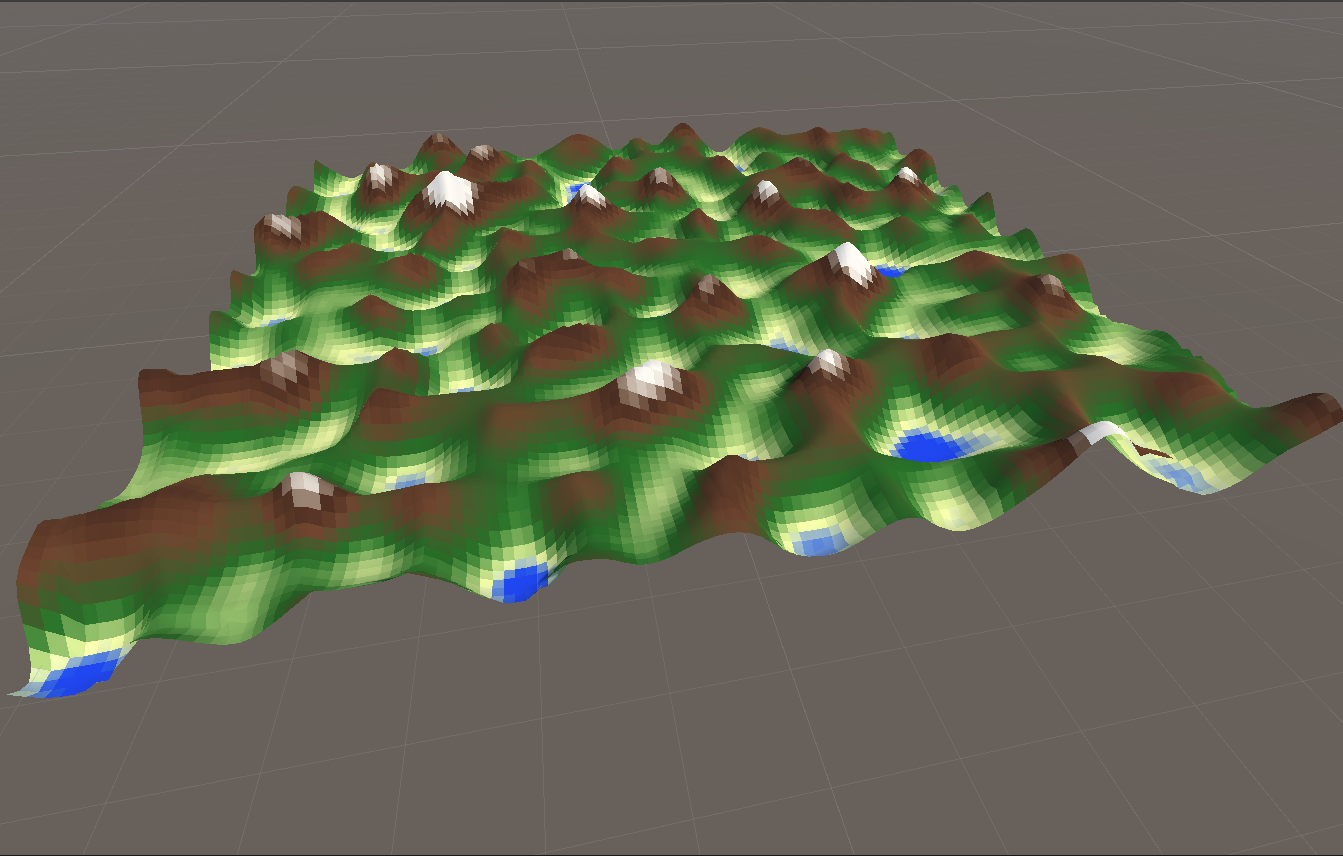
\includegraphics[width=\textwidth]{img/3ciclos.png}
        \caption{3 Ciclos de erosión con ángulo de talud de 0 grados}
    \end{minipage}
    
    \vspace{0.5cm} % Espacio vertical entre las dos filas de imágenes
    
    \begin{minipage}{0.4\textwidth}
        \centering
        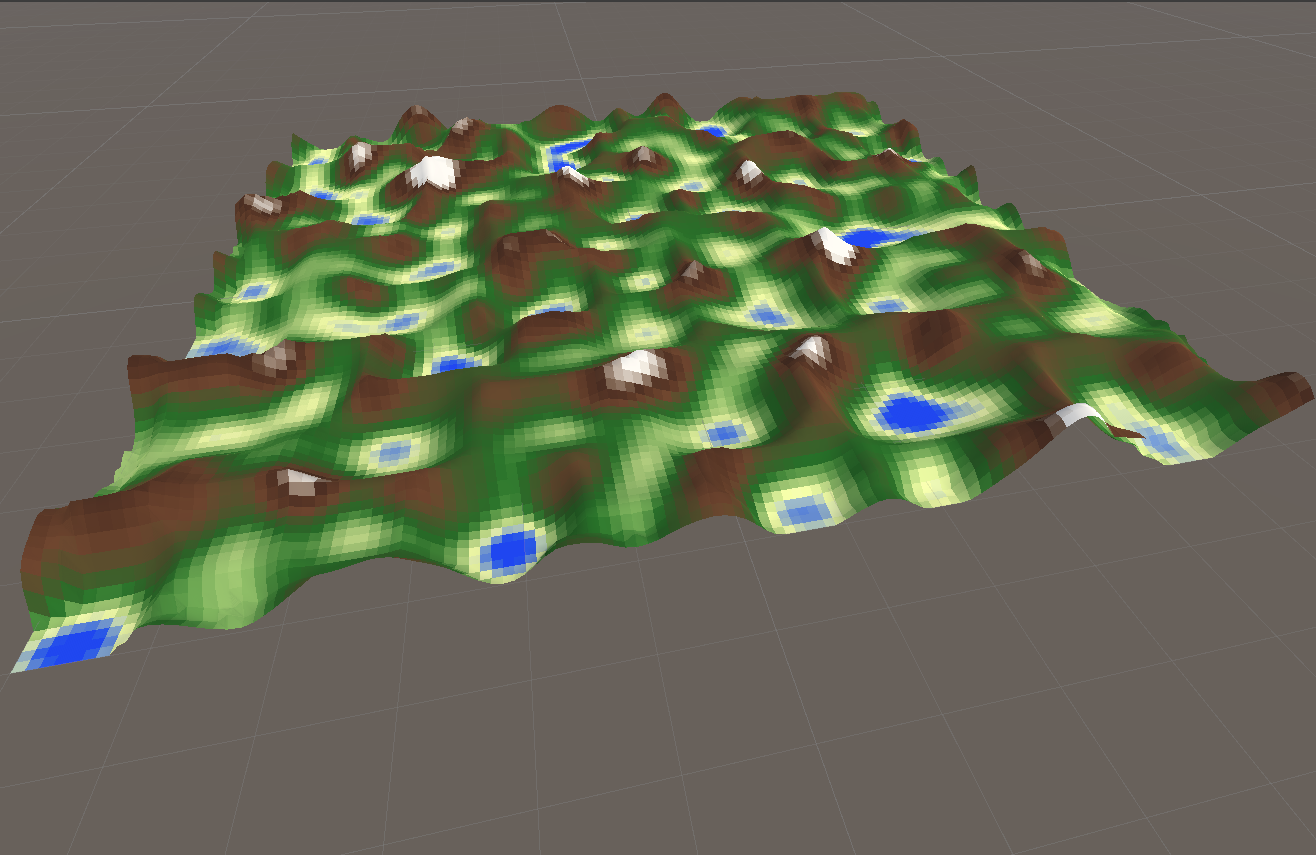
\includegraphics[width=\textwidth]{img/7ciclos.png}
        \caption{7 Ciclos de erosión con ángulo de talud de 0 grados}
    \end{minipage}%
    \hfill
    \begin{minipage}{0.4\textwidth}
        \centering
        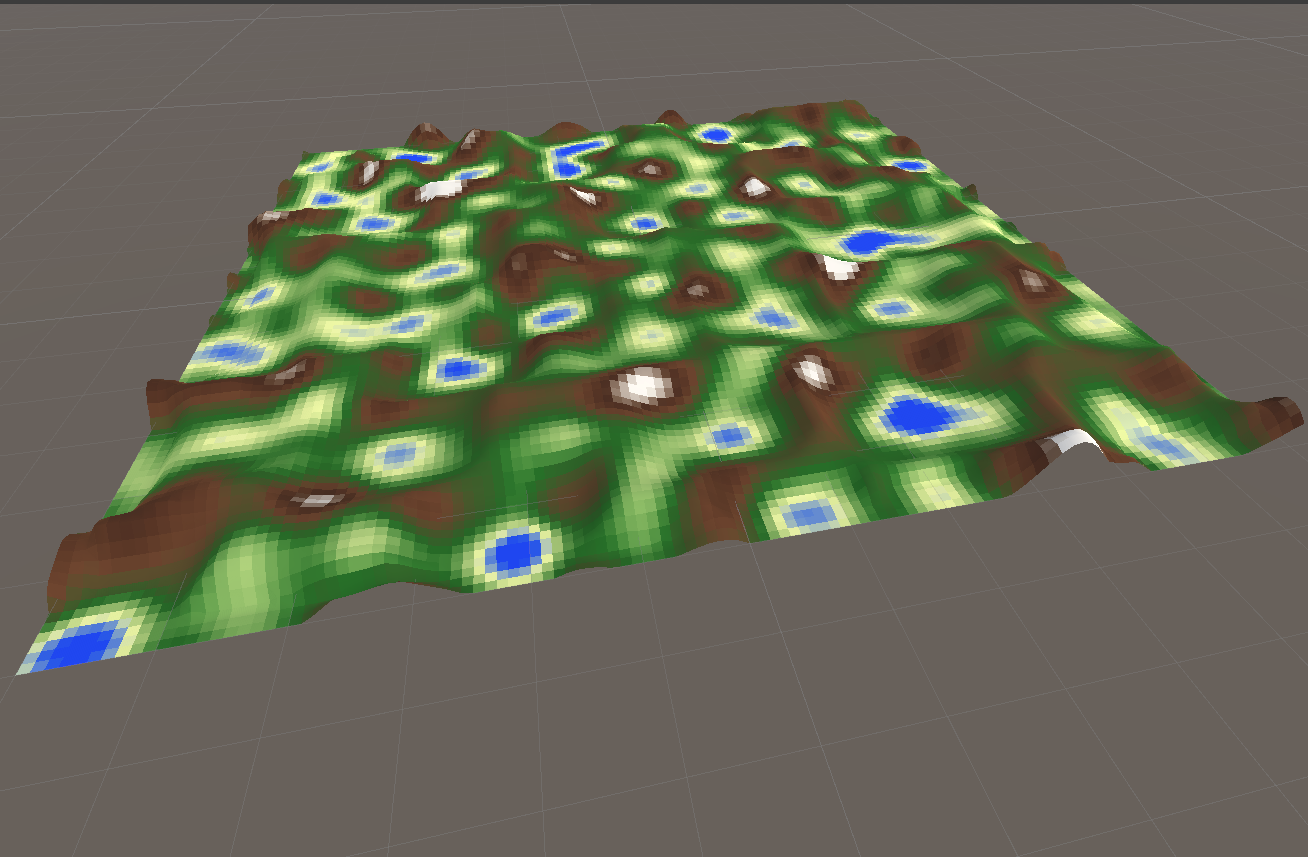
\includegraphics[width=\textwidth]{img/12ciclos.png}
        \caption{12 Ciclos de erosión con ángulo de talud de 0 grados}
    \end{minipage}
    \caption{Comparación del efecto de diferentes ciclos de erosión}
\end{figure}

Como se puede ver en la figura, cuanto mayor es el número de ciclos, más erosionado y liso queda el terreno.

\subsubsection{Ángulo de talud: }El ángulo de talud es el ángulo mínmo que tiene que haber entre la recta que une dos alturas y la horizontal para que produzca erosion entre ellas. A menor sea el ángulo, mayor erosión habrá por cada iteración.

A continuación, se mostrará otra tabla como la anterior donde se podrán ver los efecto de un angulo de talud mayor cada vez para un númeor igual de ciclos.
\begin{figure}[ht]
    \centering
    \begin{minipage}{0.45\textwidth}
        \centering
        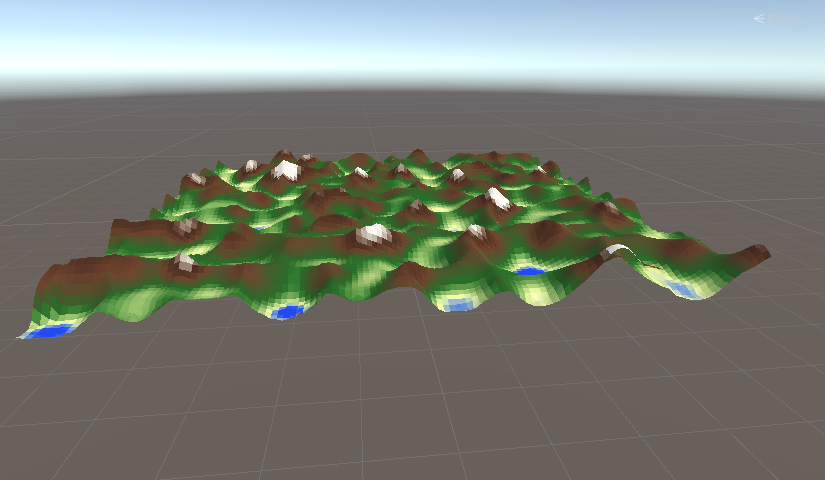
\includegraphics[width=\textwidth]{img/talud0.png}
        \caption{5 Ciclos de erosión con ángulo de talud de 0 grados}
    \end{minipage}%
    \hfill
    \begin{minipage}{0.45\textwidth}
        \centering
        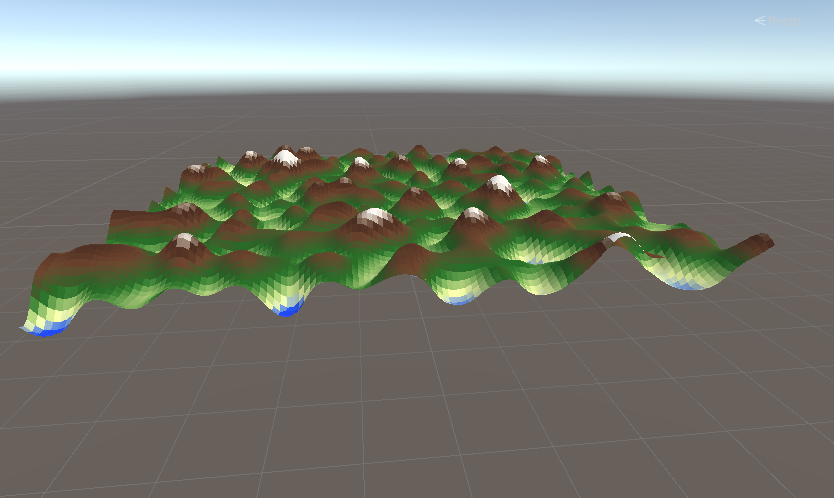
\includegraphics[width=\textwidth]{img/talud30.png}
        \caption{5 Ciclos de erosión con ángulo de talud de 30 grados}
    \end{minipage}
    
    \vspace{0.5cm} % Espacio vertical entre las dos filas de imágenes
    
    \begin{minipage}{0.45\textwidth}
        \centering
        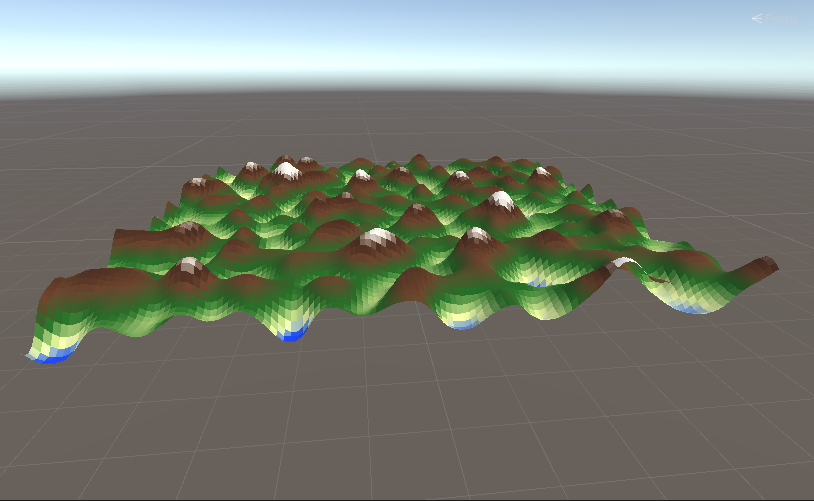
\includegraphics[width=\textwidth]{img/talud60.png}
        \caption{5 Ciclos de erosión con ángulo de talud de 60 grados}
    \end{minipage}%
    \hfill
    \begin{minipage}{0.45\textwidth}
        \centering
        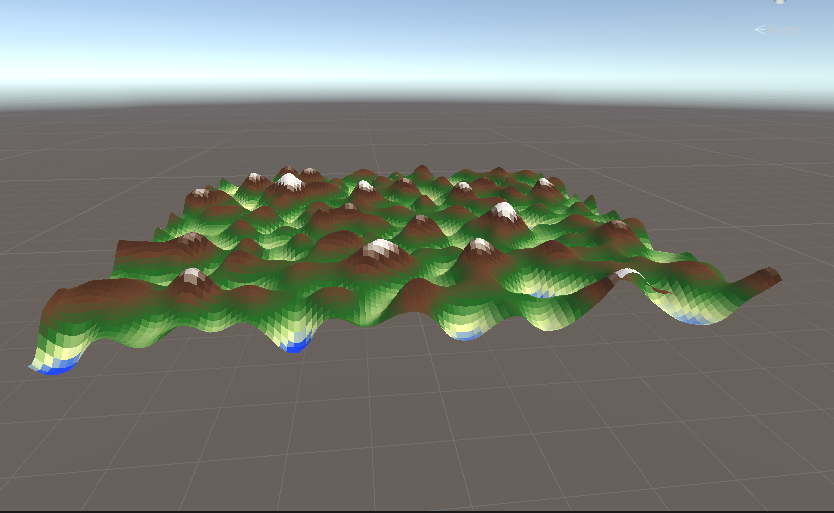
\includegraphics[width=\textwidth]{img/talud90.png}
        \caption{5 Ciclos de erosión con ángulo de talud de 90 grados}
    \end{minipage}
    \caption{Comparación del efecto de diferentes ciclos de erosión}
\end{figure}

\subsubsection{Border Size y Border Max Reduction: }Border size es una variable que sirve para dar continuidad a los bordes de los chunks cuando sufren erosion. De esta manera aunque los chunks modifiquen su mapa de alturas interno en base a sus alturas relativas, los bordes se mantendrán intactos y mantendrán la continuidad unos con otros. No obstante esto puede provocar que os bordes queden muy pronunciados si se produce mucha erosión e el interior de los chunks, es por esto que se ha tratado de redudir la altura de los bvordes uniformemente con el parámetero Border Max Reduction, el cual hace que en cada iteración, se reduzca un poco el borde para dar coherencia al terrneo.

A continuación se muestra como afecta la combinación de estos dos factores:
\begin{figure}[ht]
    \centering
    \begin{minipage}{0.4\textwidth}
        \centering
        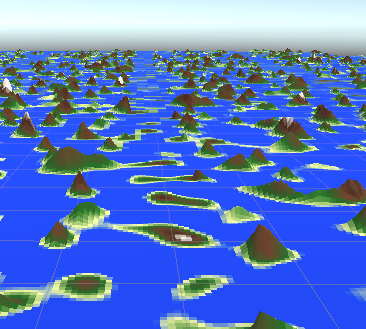
\includegraphics[width=\textwidth]{img/hightbordersize-hightborderred.png}
        \caption{Border Size grande, Reducción de borde grande}
    \end{minipage}%
    \hfill
    \begin{minipage}{0.4\textwidth}
        \centering
        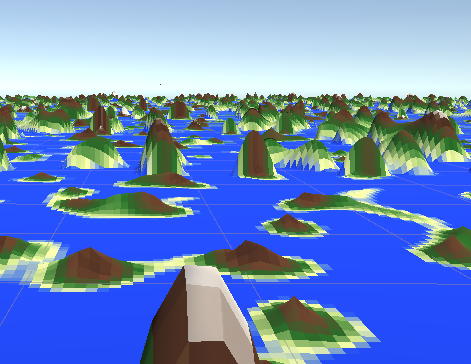
\includegraphics[width=\textwidth]{img/hightbordersize-lowborderred.png}
        \caption{Border Size grande, Reducción de borde baja}
    \end{minipage}
    
    \vspace{0.5cm} % Espacio vertical entre las dos filas de imágenes
    
    \begin{minipage}{0.4\textwidth}
        \centering
        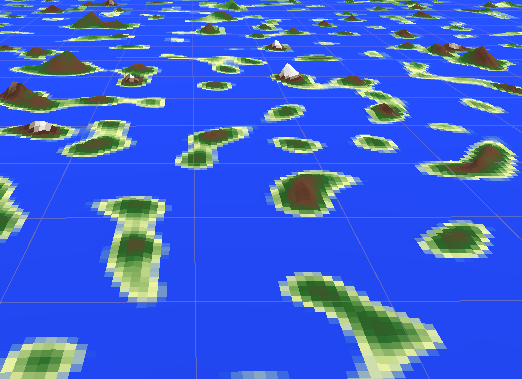
\includegraphics[width=\textwidth]{img/lowbordersize-hightborderred.png}
        \caption{Border Size baja, Reducción de borde grande}
    \end{minipage}%
    \hfill
    \begin{minipage}{0.4\textwidth}
        \centering
        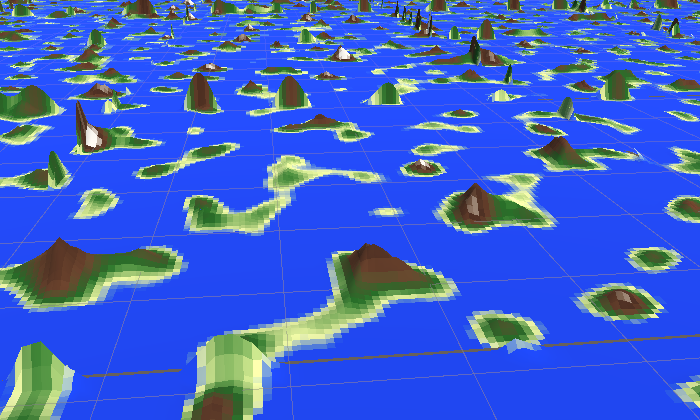
\includegraphics[width=\textwidth]{img/lowbordersize-lowborderred.png}
        \caption{Border Size baja, Reducción de borde baja}
    \end{minipage}
    \caption{Comparación del efecto de la combinación de los border size y border max reduction}
\end{figure}

La elección del tamaño del borde y la cantidad de ciclos de erosión tiene un impacto en la apariencia del terreno generado. Un borde grande puede crear un efecto de "pasillo" entre los trozos del terreno al reducir drásticamente el borde en cada iteración de erosión. Un borde pequeño puede hacer que cada trozo esté "enmarcado" por los vértices del borde original, especialmente cuando se realizan múltiples ciclos de erosión.

La combinación de estos parámetros debe ser cuidadosamente considerada para lograr un nivel de altura promedio coherente en el terreno, evitando que se perciba una frontera visible entre los trozos del terreno.

\section{Visualización}
\subsection{Representación Gráfica}

En esta subsección, se presentarán imágenes y representaciones gráficas del terreno generado utilizando tres algoritmos diferentes: Perlin, Simplex y Voronoi. Cada algoritmo producirá visualizaciones en diferentes modos, como mapa de ruido, mapa de colores y malla 3D.

\begin{itemize}
   \item \subsubsection{Algoritmo Perlin:}
   \begin{figure}[htbp]
    \begin{minipage}[t]{0.3\linewidth}
        \centering
        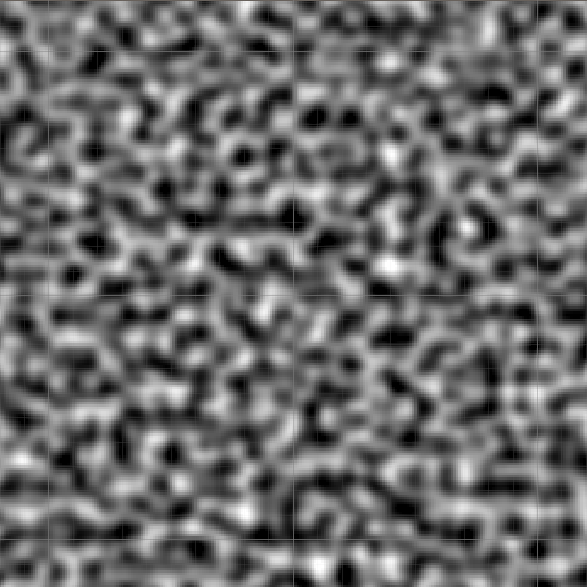
\includegraphics[width=\textwidth, height=4cm]{img/codes/Perlin123.png}
        \caption{Mapa de Ruido (Perlin)}
    \end{minipage}%
    \hfill
    \begin{minipage}[t]{0.3\linewidth}
        \centering
        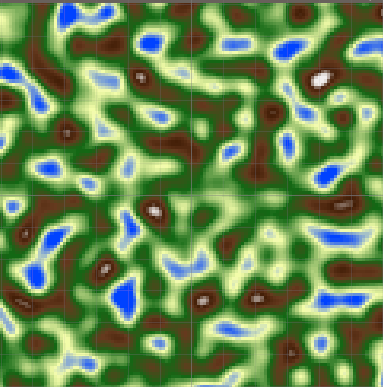
\includegraphics[width=\textwidth, height=4cm]{img/codes/PerlinColores.png}
        \caption{Mapa de Colores (Perlin)}
    \end{minipage}%
    \hfill
    \begin{minipage}[t]{0.3\linewidth}
        \centering
        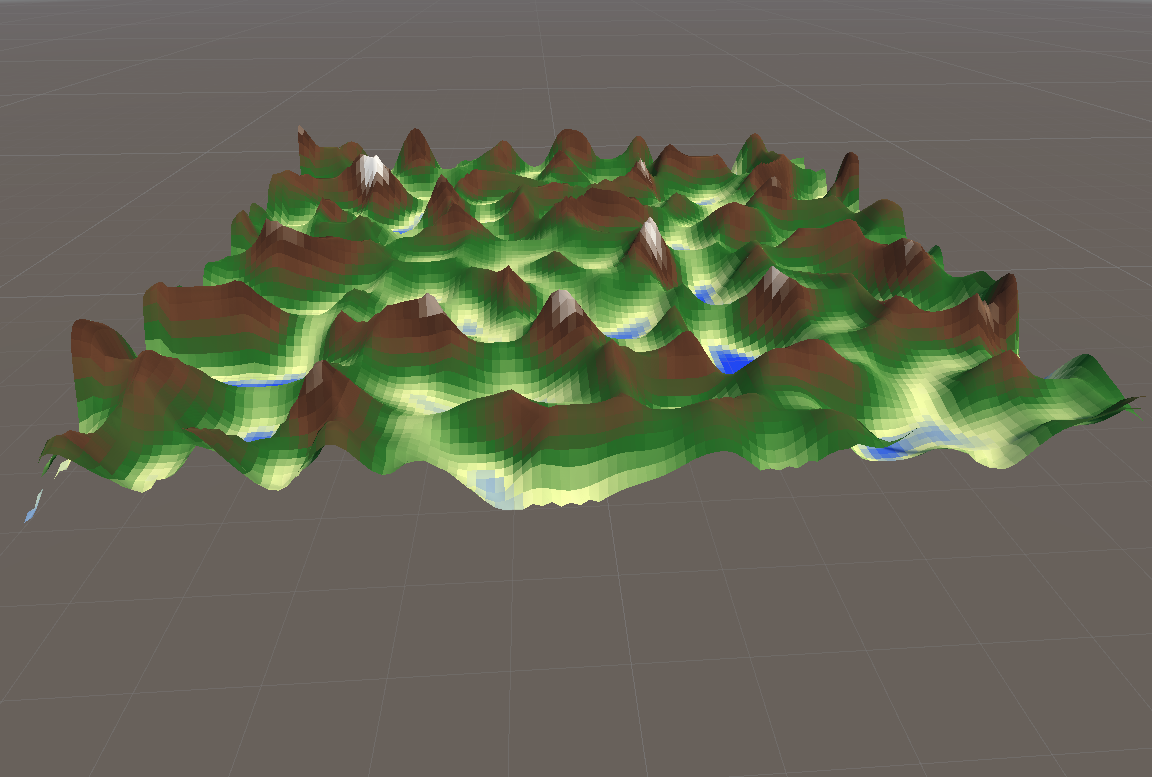
\includegraphics[width=\textwidth, height=4cm]{img/codes/Perlin3D.png}
        \caption{Malla 3D (Perlin)}
    \end{minipage}
    
    \end{figure}
    
    
    \item \subsubsection{Algoritmo Simplex:}
    
    \begin{figure}[htbp]
        \begin{minipage}[t]{0.3\linewidth}
            \centering
            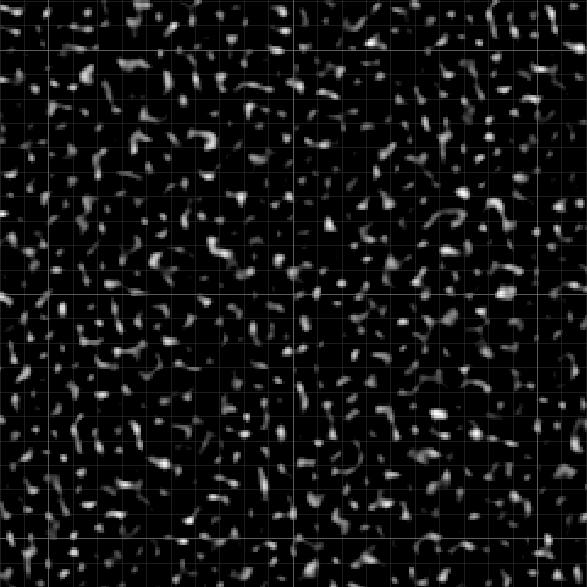
\includegraphics[width=\textwidth, height=4cm]{img/codes/Simplex123.png}
            \caption{Mapa de Ruido (Simplex)}
        \end{minipage}%
        \hfill
        \begin{minipage}[t]{0.3\linewidth}
            \centering
            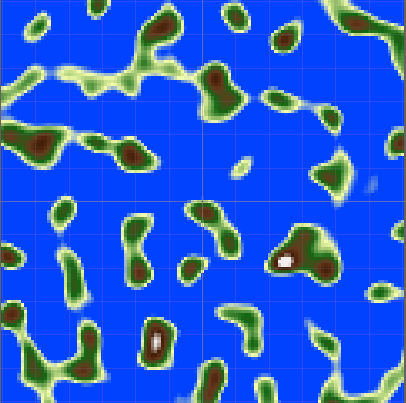
\includegraphics[width=\textwidth, height=4cm]{img/codes/SimplexColors.png}
            \caption{Mapa de Colores (Simplex)}
        \end{minipage}%
        \hfill
        \begin{minipage}[t]{0.3\linewidth}
            \centering
            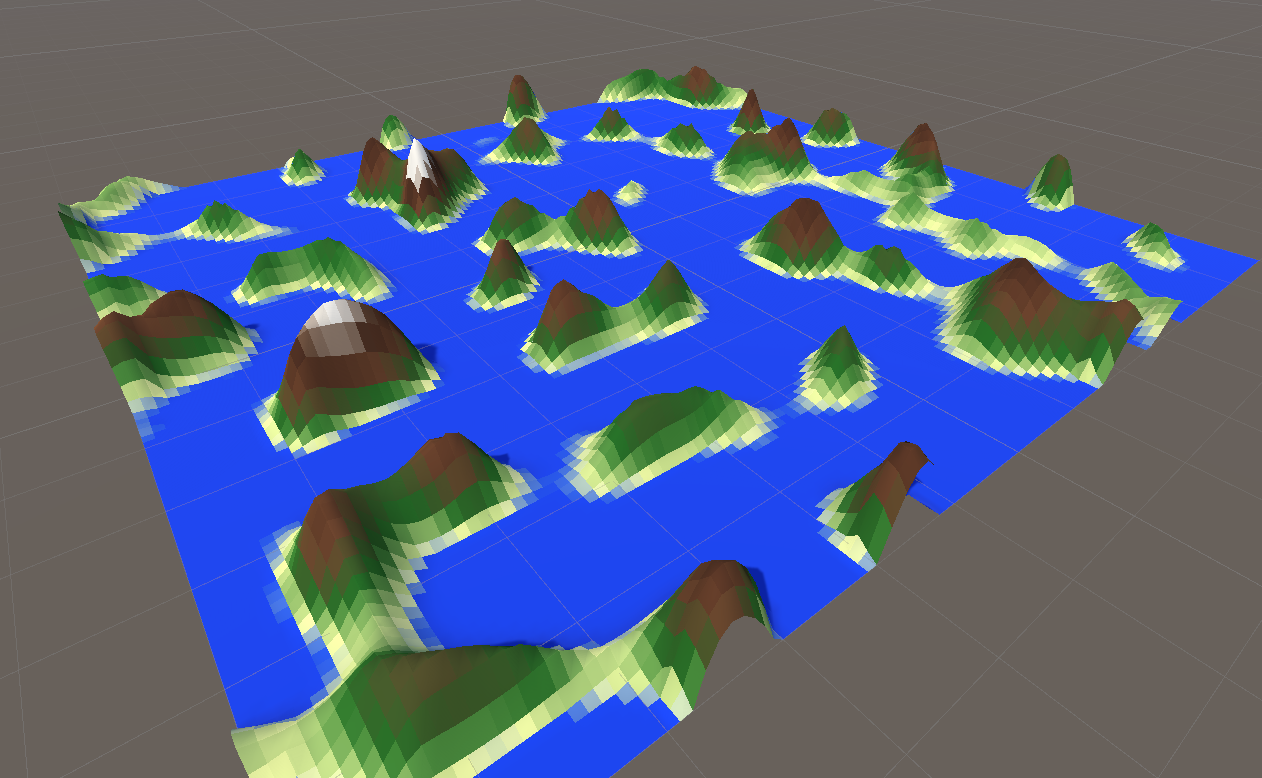
\includegraphics[width=\textwidth, height=4cm]{img/codes/Simples3D.png}
            \caption{Malla 3D (Simplex)}
        \end{minipage}
        
    \end{figure}
    
    \item \subsubsection{Algoritmo Voronoi:}
    
    \begin{figure}[htbp]
        \begin{minipage}[t]{0.3\linewidth}
            \centering
            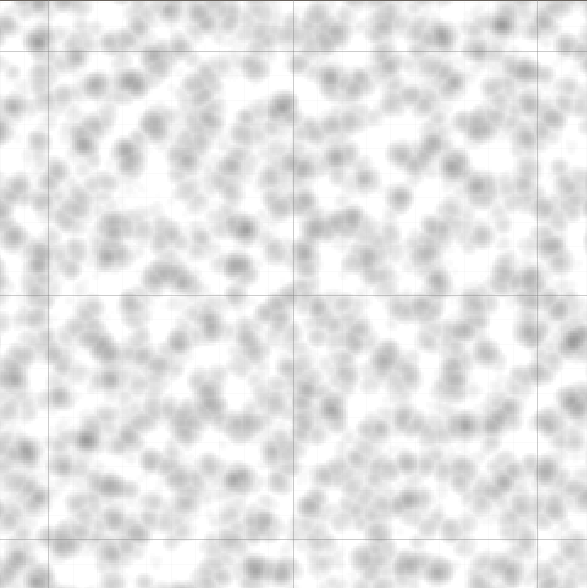
\includegraphics[width=\textwidth, height=4cm]{img/codes/Voronoi123.png}
            \caption{Mapa de Ruido (Voronoi)}
        \end{minipage}%
        \hfill
        \begin{minipage}[t]{0.3\linewidth}
            \centering
            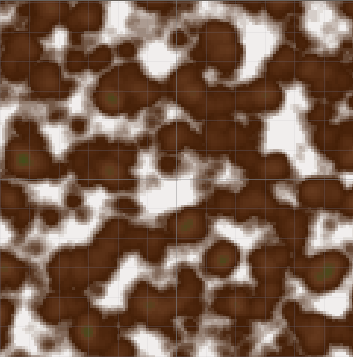
\includegraphics[width=\textwidth, height=4cm]{img/codes/VoronoiColores.png}
            \caption{Mapa de Colores (Voronoi)}
        \end{minipage}%
        \hfill
        \begin{minipage}[t]{0.3\linewidth}
            \centering
            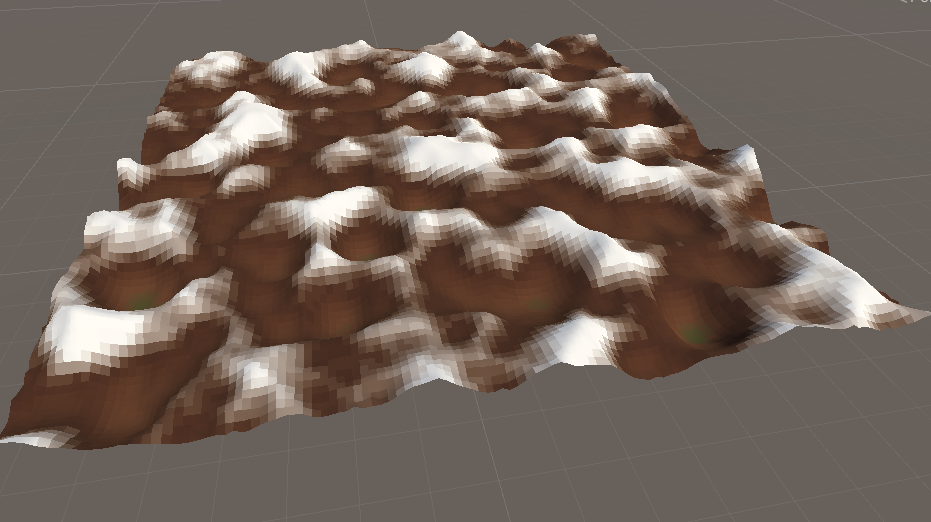
\includegraphics[width=\textwidth, height=4cm]{img/codes/Voronoi3D.png}
            \caption{Malla 3D (Voronoi)}
        \end{minipage}
        
    \end{figure}
\end{itemize}

Estas visualizaciones proporcionan una representación completa de cómo se ve el terreno generado utilizando diferentes algoritmos y modos de representación.

\subsection{Comparación de LOD}

En esta sección se presenta una comparación visual de los diferentes niveles de detalle (LOD) utilizados en la representación del terreno. Se mostrarán imágenes que ilustran cómo varía la calidad visual a medida que se ajusta el nivel de detalle.

\begin{itemize}
    \item \textbf{Vista superior: } Imágenes del LOD visto desde arriba:
    \begin{figure}[h]
        \begin{minipage}{0.45\textwidth}
            \centering
            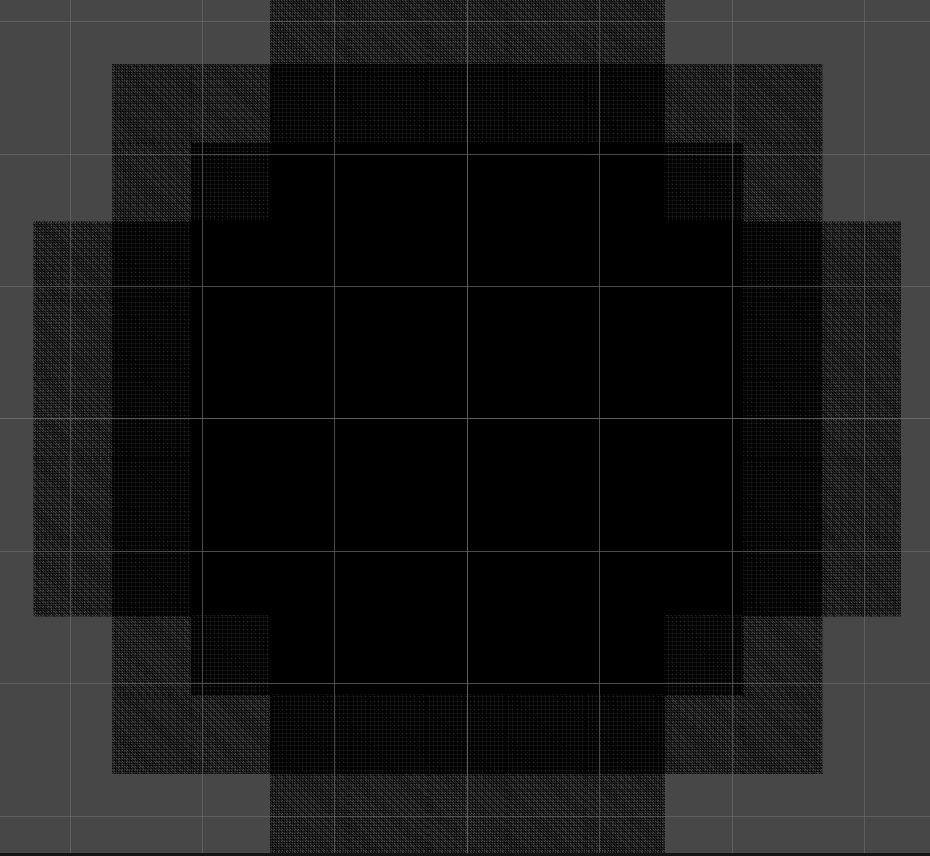
\includegraphics[width=\textwidth]{img/codes/FlyViewLOD.png}
            \caption{Vista general del LOD}
        \end{minipage}%
        \hfill
        \begin{minipage}{0.45\textwidth}
            \centering
            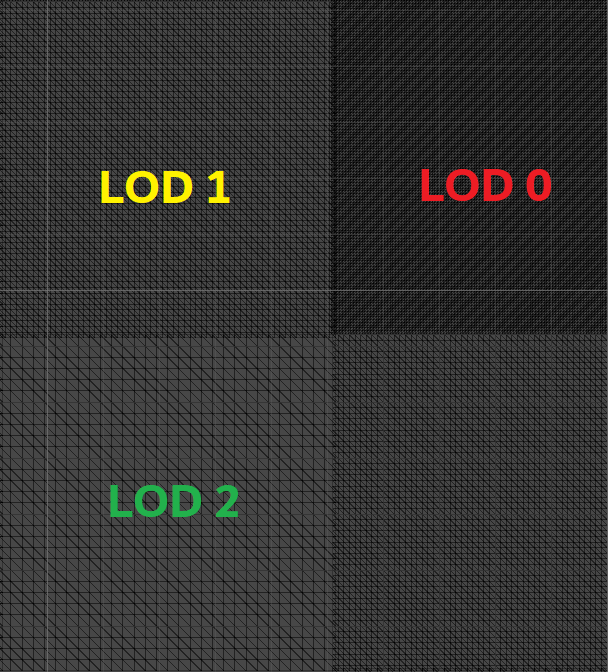
\includegraphics[width=\textwidth]{img/codes/3LOD.png}
            \caption{Vista de los 3 LOD juntos}
        \end{minipage}
    \end{figure}

    \item \textbf{Vista individual: } tres imágenes individuales que muestran cada nivel de detalle (LOD) por separado:
    \begin{figure}[h]
        \begin{minipage}{0.3\textwidth}
            \centering
            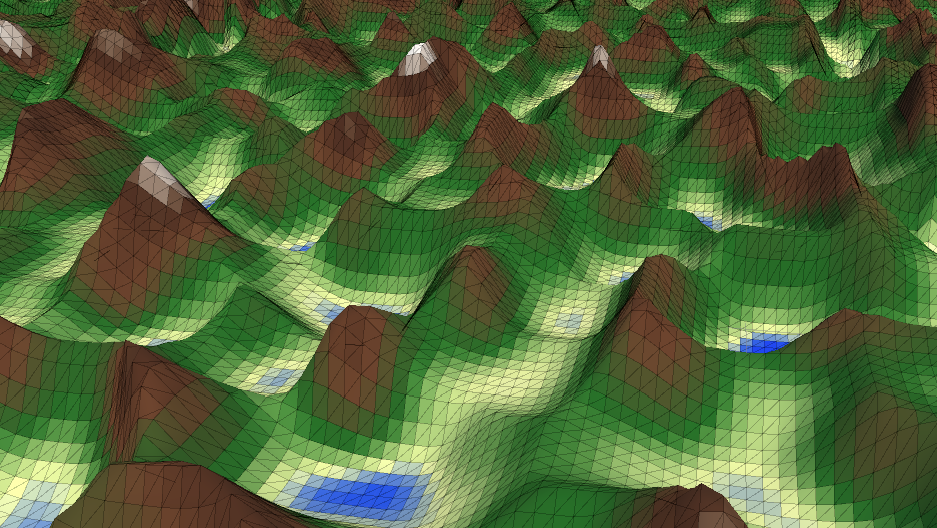
\includegraphics[width=\textwidth]{img/codes/LOD0.png}
            \caption{LOD 0}
        \end{minipage}%
        \hfill
        \begin{minipage}{0.3\textwidth}
            \centering
            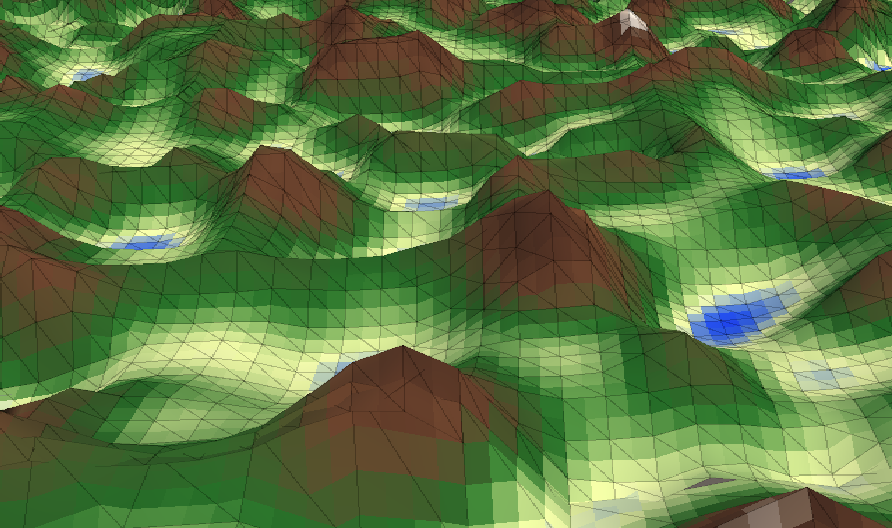
\includegraphics[width=\textwidth]{img/codes/LOD1.png}
            \caption{LOD 1}
        \end{minipage}
        \hfill
        \begin{minipage}{0.3\textwidth}
            \centering
            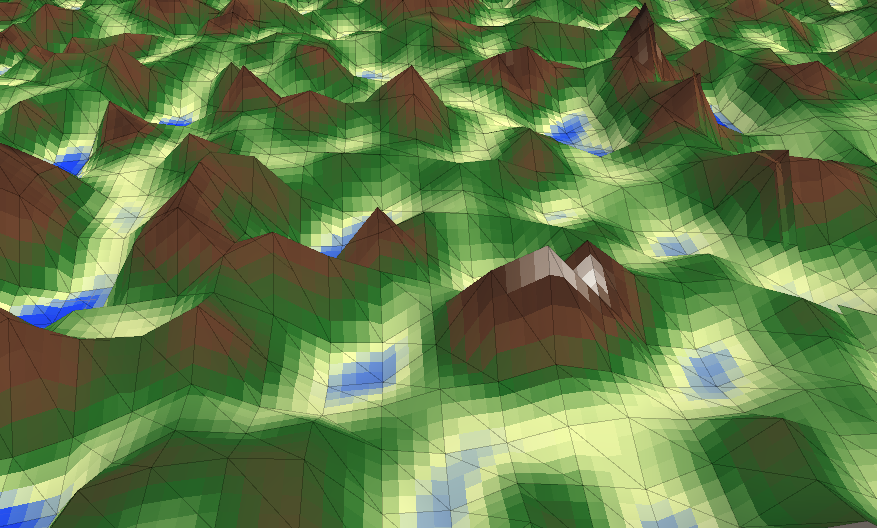
\includegraphics[width=\textwidth]{img/codes/LOD2.png}
            \caption{LOD 2}
        \end{minipage}
    \end{figure}
\end{itemize}

Estas imágenes permiten apreciar las diferencias en la calidad y detalle del terreno en función del nivel de detalle seleccionado.


% \section{Rendimiento}

% \subsection{Tiempo de Generación de Terreno}

% Se realizarán pruebas de rendimiento para medir el tiempo necesario para generar un terreno con diferentes configuraciones. Se analizará cómo la paralelización de tareas afecta el rendimiento en sistemas multicore.

% \subsection{Optimización de Malla}

% Se evaluará el impacto de las técnicas de optimización, como el LOD (Niveles de Detalle) y el almacenamiento en caché, en el rendimiento de la aplicación. Se compararán las tasas de fotogramas (FPS) en diferentes configuraciones de malla.

% \section{Conclusión del Análisis}

% En esta sección final del capítulo, se resumirán los resultados clave del análisis y se discutirán las conclusiones obtenidas. Se destacarán los logros del proyecto, las lecciones aprendidas y las posibles mejoras futuras.

